\documentclass[11pt]{article}
\usepackage[a4paper,margin=2cm]{geometry}
\usepackage[T1]{fontenc}
\usepackage{amsmath,amssymb}
\usepackage{graphicx}
\usepackage{booktabs}
\usepackage{subcaption}
\usepackage{caption}
\usepackage{microtype}
\usepackage{enumitem}
\usepackage{titlesec}
\usepackage[hidelinks]{hyperref}
\usepackage{xcolor}

\graphicspath{{figures/}}
\captionsetup{font=small,labelfont=bf,skip=3pt}
\setlist[itemize]{nosep,leftmargin=1.4em,topsep=1pt}
\titleformat{\section}{\normalfont\large\bfseries}{}{0pt}{}
\titlespacing*{\section}{0pt}{1.3ex plus .2ex}{0.6ex}
\setlength{\parindent}{0pt}\setlength{\parskip}{2.5pt}
\tolerance=2000 \emergencystretch=3em \hbadness=2000
\usepackage[htt]{hyphenat}
\hypersetup{colorlinks=true,urlcolor=blue!55!black,linkcolor=blue!55!black}

\newcommand{\wb}[1]{\href{https://wandb.ai/sichengma0514-university-of-cambridge/a8-grpo/runs/#1}{\texttt{#1}}}
\newcommand{\axv}[2]{\href{https://arxiv.org/abs/#1}{#2}}
\newcommand{\code}[1]{\texttt{#1}}

\begin{document}
\begin{center}
  {\Large\bfseries Part I --- GRPO Finetuning of \texttt{gemma-3-1b-it} on GSM8K}\\[3pt]
  {Multi-Agent Systems and Agentic AI --- Practical Examination}\\[5pt]
  {\small Team \textbf{chmawa} (sm3035, bc654, zw499)\quad$\cdot$\quad written individually by Zixuan Wang (zw499)}\\[3pt]
  {\small\itshape Jointly owned (shared team work): the v6e-1 TPU, the seven shared GRPO runs (\texttt{bdbugenj} and R0--R5), and the code repository.
  All prose, figure selection and interpretation below are my own.}\\[3pt]
  {\small Code: \href{https://github.com/wdk0082/a8-grpo}{\texttt{github.com/wdk0082/a8-grpo}} \emph{(to be ported to GitLab for submission)}\;$\mid$\;
  W\&B: \href{https://wandb.ai/sichengma0514-university-of-cambridge/a8-grpo}{\texttt{a8-grpo}}\;$\mid$\;
  \axv{2402.03300}{GRPO}, \axv{2503.14476}{DAPO}, \axv{2106.09685}{LoRA}, \href{https://huggingface.co/datasets/openai/gsm8k}{GSM8K}}
\end{center}
\vspace{1pt}\hrule\vspace{4pt}

\section*{I.1\quad Reproducing the baseline}
\textbf{(i) The run.} Shared baseline run (\wb{bdbugenj}): upstream commit
\href{https://github.com/borisbolliet/tpu-2026}{\texttt{borisbolliet/tpu-2026@77c5a67}}, unmodified \code{config.py},
full \textbf{3364} GRPO steps (one epoch), \textbf{4\,h\,43\,m} wall-clock on \code{v6e-1}.

\textbf{(ii) Accuracy.} GSM8K \emph{test} split (materialised from TFDS, shuffle seed 42, $n{=}64$, greedy, exact numeric match).
Base \code{gemma-3-1b-it}: \textbf{51.6\%}; LoRA checkpoint \textbf{28.1\%} at its best \emph{surviving} step (2000; \code{bdbugenj}'s earlier, better checkpoints were pruned) and \textbf{3.1\%} at step 3364.
The baseline \emph{over-optimises}: exact-match correctness falls $52\!\to\!28\!\to\!6\!\to\!3$\% across steps $0/2000/3000/3364$ while the
format-shaping reward saturates (it reward-hacks the template). At $n{=}64$ the CI is $\pm12$\,pt, so we firm the base figure to
\textbf{47.4\%} on the full 1319-example test in I.3.

\textbf{(iii) Training curves.} Fig.~\ref{fig:rewardkl} (grey = baseline): mean reward $\bar r$ peaks $\approx$\,step 450 then declines, and
$\mathrm{KL}(\pi_\theta\Vert\pi_{\mathrm{ref}})$ rises $0.16\!\to\!{\sim}0.5$ with late spikes --- the textbook over-optimisation arc.

\textbf{Baseline patches} (as-shipped fixes; full diff: \code{tpu-2026\_our\_changes.patch} in repo).
(1) \code{run\_tmux.sh} hard-coded a foreign home path; (2) the W\&B entity defaulted to a third party --- redirected to \code{a8-grpo};
(3) \code{evaluate.py} built a fresh $B{=}0$ LoRA and never restored a checkpoint, so it could only score \emph{base} --- we added Orbax
\code{--step}/\code{--ckpt-dir} LoRA restore; (4) TFDS's gsm8k builder crashes under protobuf 7.x once JAX imports, so we pre-materialise
the seed-42 test split (\code{prepare\_test\_tfds.py}) and added an HF \code{datasets} fallback.

\section*{I.2\quad Understanding the baseline}
\textbf{(a) Policies \& trainable parameters.} $\pi_\theta$ is the LoRA-adapted policy: frozen \code{gemma-3-1b-it} weights plus low-rank
adapters $\Delta W{=}BA$; \textbf{only $A,B$ are trainable} (the base is frozen). $\pi_{\mathrm{old}}$ is the policy that generated the current
rollouts --- with \code{NUM\_ITERATIONS} $\mu{=}1$ there is one gradient step per rollout batch, so $\pi_{\mathrm{old}}{=}\pi_\theta$ at the update.
$\pi_{\mathrm{ref}}$ is the frozen initial policy for the KL penalty; LoRA initialises $B{=}0$, so $\pi_\theta{=}\pi_{\mathrm{ref}}$ exactly at step 0.

\textbf{(b) Group size \& estimator.} $K{=}$\code{NUM\_GENERATIONS}$=2$. Tunix uses \code{advantage\_estimator='grpo'}: the \textbf{standard}
group-mean, std-normalised advantage $\hat A_i{=}(r_i-\bar r)/\sigma_r$ with $\bar r,\sigma_r$ over all $K$ samples \emph{including} $i$ --- \emph{not}
leave-one-out.

\textbf{(c) Shaping vs.\ correctness rewards.} Shaping: \code{match\_format\_exactly} and \code{match\_format\_approximately} (reward the
\code{<reasoning>}/\code{<answer>} template). True correctness: \code{check\_answer} and \code{check\_numbers} (extracted number vs.\ gold).
With the correctness reward \emph{alone}, an early policy is almost never numerically right, so every sample in a group scores $\approx 0$:
within-group $\sigma_r\!\to\!0$ and $\hat A_i{=}(r_i-\bar r)/\sigma_r$ has no signal (an $\varepsilon$ in the denominator averts a literal $0/0$) --- degenerate groups, no gradient. The shaping terms give
differently-formatted samples different rewards, restoring $\sigma_r>0$ and a usable advantage that bootstraps learning (the same
$\sigma_r\!\to\!0$ degeneracy analysed in I.4 Q1).

\textbf{(d) Clipped surrogate \& $\epsilon$.} The PPO-style clip lives in Tunix's \code{GRPOLearner} (module \code{tunix.rl}), in its clipped policy-gradient loss: it forms a
\textbf{per-token} ratio $\rho_t{=}\pi_\theta(a_t)/\pi_{\mathrm{old}}(a_t)$ and optimises $\min\!\big(\rho_t\hat A,\ \mathrm{clip}(\rho_t,1{-}\epsilon,1{+}\epsilon)\hat A\big)$,
with $\epsilon{=}$\code{EPSILON}$=0.2$. Two deviations from the lecture form: (i) the ratio is \textbf{per-token}, not per-sequence; (ii) at
$\mu{=}1$, $\pi_{\mathrm{old}}{=}\pi_\theta\Rightarrow\rho_t\equiv1$, so the clip is \textbf{dormant} in the baseline (it engages only for $\mu>1$).

\section*{I.3\quad Improving on the baseline}
\textbf{Modification \& motivation.} The baseline over-optimises at $K{=}2$. The theory of I.4 Q1 gives the GRPO gradient variance
$\operatorname{Var}(\hat g)=K^{-2}\sum_i(h_i-\bar h)(h_i-\bar h)^\top=O(1/K)$, with effective sample size $K_{\mathrm{eff}}\!\propto\!K$: a larger
group directly lowers the variance of the gradient estimate $\hat g$. We therefore take \textbf{group size $G$} (the $K$ of I.2(b) and the theory) as the primary lever and run a controlled
$\beta\times G$ \textbf{2$\times$2} (KL-penalty weight $\times$ group size) to separate it from the KL leash:
R4$(G2,\beta0)$, R0$(G2,\beta.08$; baseline re-run$)$, R3b$(G8,\beta0)$, R5$(G8,\beta.08)$ --- plus single-axis controls R1$(\beta{=}0.3)$ and
R2$(+\text{soft length penalty})$, for \textbf{six full runs}. All share data (HF GSM8K, seed 42), eval, horizon (3364 steps) and a seed-matched
rollout RNG (\code{PRNGKey(0)}); only the named knob changes per run. R0 re-runs the baseline config with \emph{dense} checkpoints, so its best-val
$46.7\%$ recovers the peak that \code{bdbugenj}'s pruning hid behind I.1's $28.1\%$.

\begin{table}[t]
\centering\small
\caption{Held-out accuracy on the \emph{full} GSM8K test ($n{=}1319$; HF and TFDS differ only in seed-42 ordering, so at full $n$ the I.1$\to$I.3 source switch is immaterial), greedy/exact-match, $\pm$95\% bootstrap CI.
Last column: \emph{paired} bootstrap $\Delta$ vs.\ base over the shared prompts (\code{paired\_ci.py}).
$\ast$ = paired 95\% CI excludes 0; $\dagger$ = collapse. R1$(G2,\beta.3)$ and R2$(G2,+\text{len})$ fell \emph{below} base
(R1 best 37.2 / final 0.0; R2 best 32.8 / final 40.6) --- clean negative results.}
\label{tab:acc}
\begin{tabular}{llrrr}
\toprule
Model & $(G,\beta)$, step & Acc.\,(\%) & 95\% CI & $\Delta$ base (paired) \\
\midrule
Base \code{gemma-3-1b-it} & --- & 47.4 & 44.7--50.0 & --- \\
R0 (baseline re-run) & $(2,.08)$ best 700 & 46.7 & 44.0--49.4 & $-0.7$\ \,n.s. \\
R0 & $(2,.08)$ final 3364 & 6.2 & 4.9--7.5 & $-41.2^{\dagger}$ \\
R4 & $(2,0)$ best 1300 & 52.8 & 50.1--55.5 & $+5.4^{\ast}$ \\
R4 & $(2,0)$ final 3364 & 48.6 & 45.9--51.3 & $+1.2$\ \,n.s. \\
\textbf{R3b} & $(8,0)$ best 1000 & 55.7 & 53.0--58.2 & $+8.3^{\ast}$ \\
\textbf{R3b} & $(8,0)$ \textbf{final 3364} & \textbf{57.2} & 54.6--59.9 & $+9.9^{\ast}$ \\
R5 & $(8,.08)$ best 1300 & 53.4 & 50.7--56.2 & $+6.1^{\ast}$ \\
R5 & $(8,.08)$ final 3364 & 55.6 & 52.8--58.2 & $+8.2^{\ast}$ \\
\bottomrule
\end{tabular}
\end{table}

\begin{figure}[t]
\centering
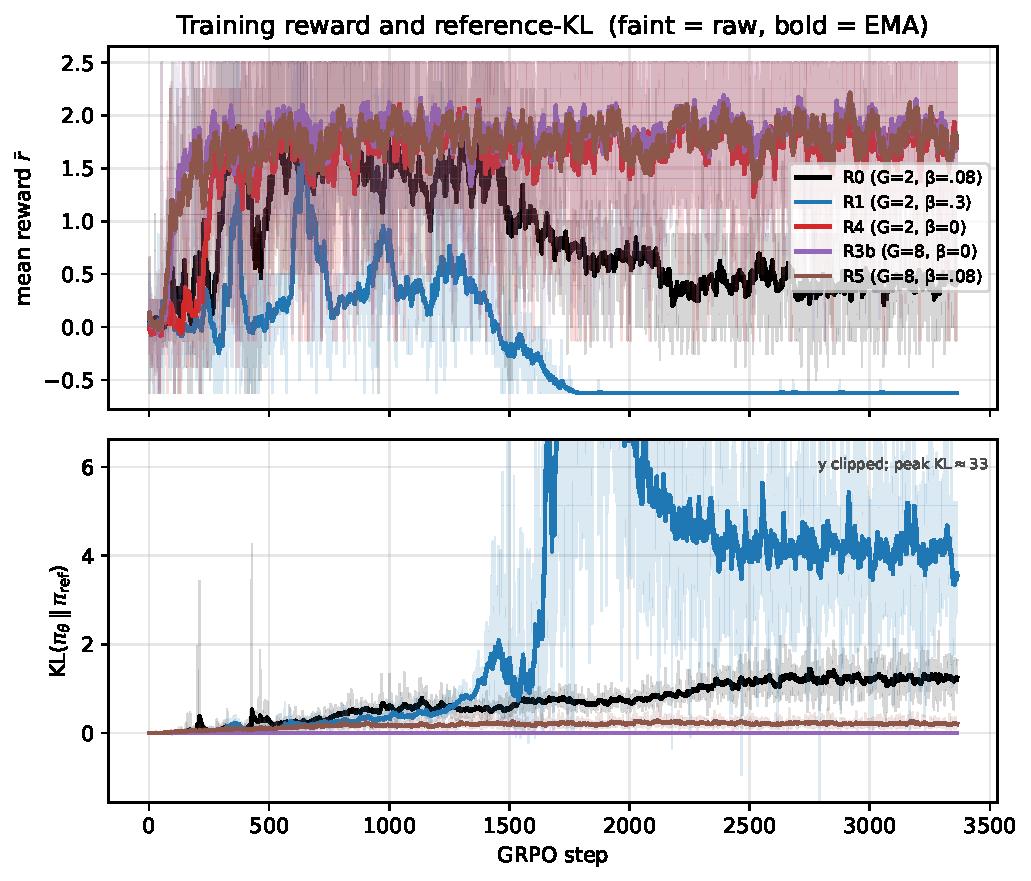
\includegraphics[width=0.86\linewidth]{F1_reward_kl.pdf}
\caption{Mean training reward $\bar r$ (top) and $\mathrm{KL}(\pi_\theta\Vert\pi_{\mathrm{ref}})$ (bottom) vs.\ GRPO step, baseline and all
variants on shared axes. Baseline/R0/R1 over-optimise (reward peaks then collapses; KL spikes); the $G{=}8$ runs (R3b, R5) and R4 stay stable.}
\label{fig:rewardkl}
\end{figure}

\begin{figure}[t]
\centering
\begin{subfigure}{0.49\linewidth}\centering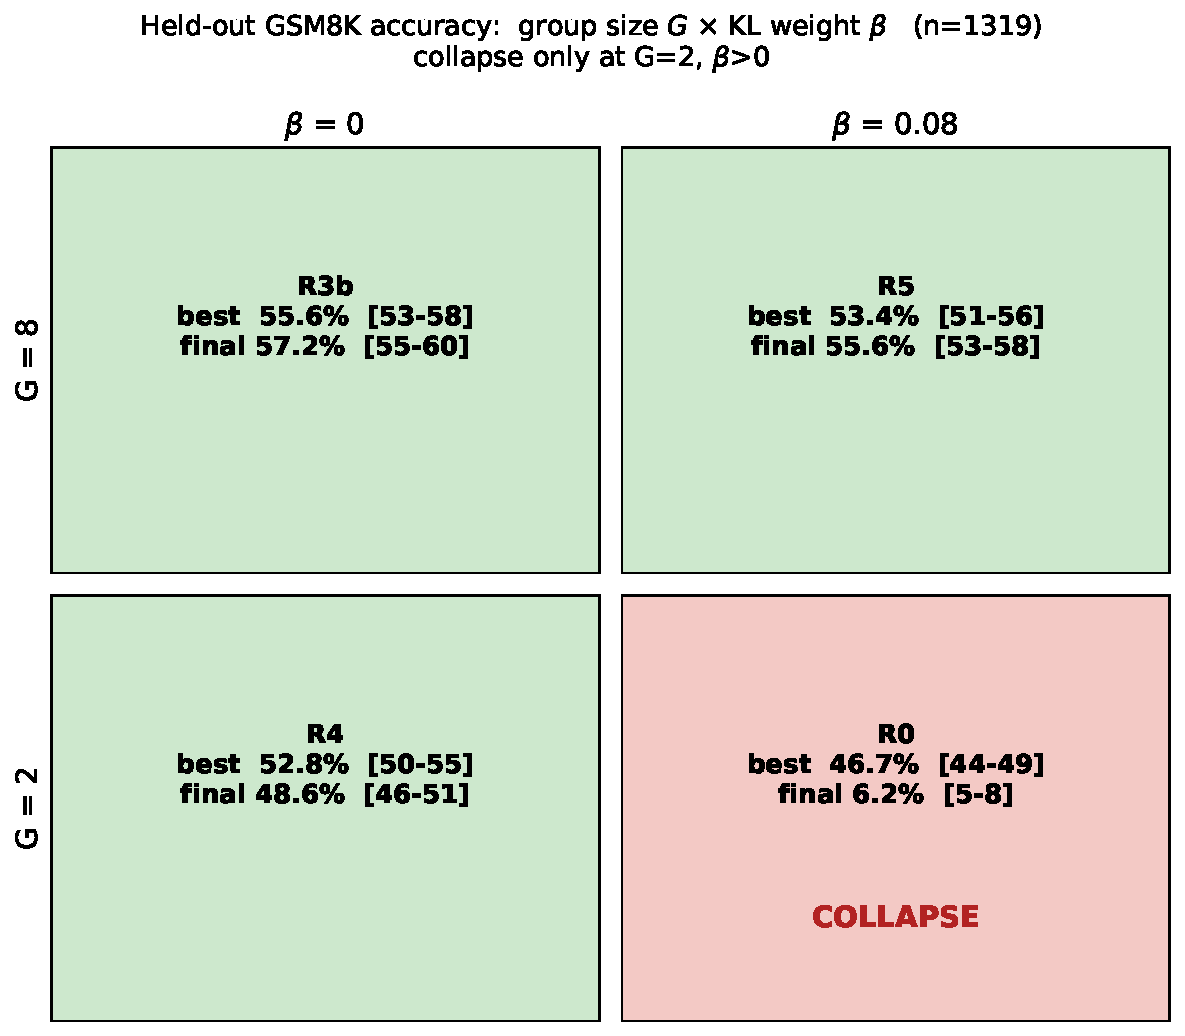
\includegraphics[width=\linewidth]{F4_2x2_GxB.pdf}\caption{$\beta\times G$ 2$\times$2 (best/final acc).}\label{fig:2x2}\end{subfigure}\hfill
\begin{subfigure}{0.49\linewidth}\centering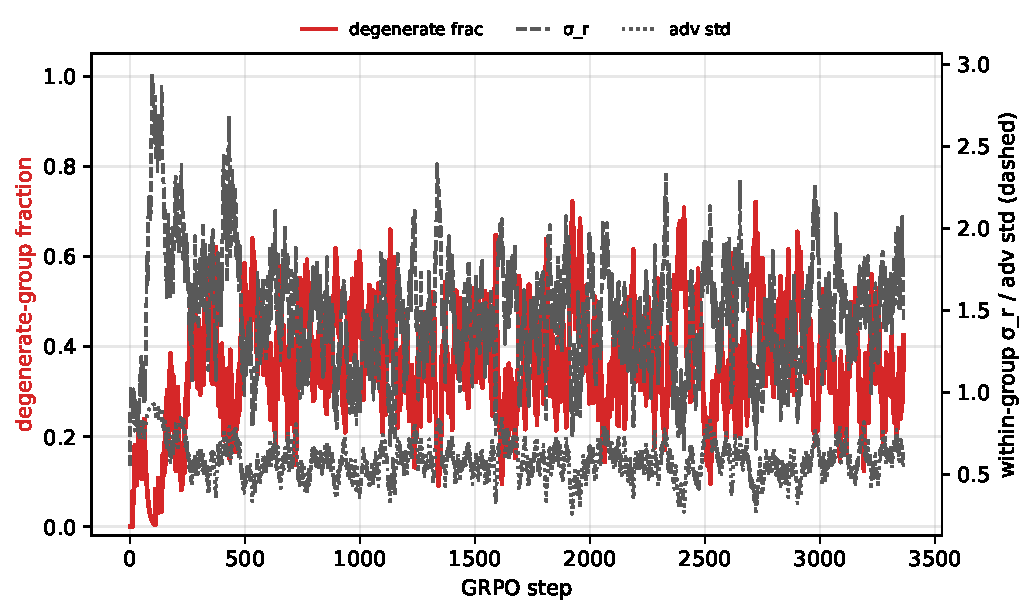
\includegraphics[width=\linewidth]{S3_group_degeneracy.pdf}\caption{Group degeneracy at $G{=}8$.}\label{fig:diag}\end{subfigure}
\caption{\emph{Left:} accuracy by $(G,\beta)$ --- collapse occurs \emph{only} at $G{=}2,\beta{>}0$ (R0). \emph{Right:} the diagnostic --- at $G{=}8$ about a
third of groups are degenerate (all-$K$ rewards equal) yet $\sigma_r$ holds $\approx1.5$ (steady, not $\to0$).}
\end{figure}

We report \textbf{(a)} held-out accuracy (Table~\ref{tab:acc}), \textbf{(b)} mean reward and KL for all runs on shared axes (Fig.~\ref{fig:rewardkl}), and \textbf{(c)} a diagnostic for a known GRPO failure mode --- group degeneracy at $G{=}8$ (Fig.~\ref{fig:diag}).

\textbf{(d) Findings vs.\ theory.} \emph{$G{=}8$ is the winning intervention.} Both $G{=}8$ runs beat base --- R3b $+9.9$, R5 $+8.2$\,pp, paired CIs
excluding 0 --- and each beats its matched $G{=}2$ run (R3b$-$R4 $=+8.6$\,pp at final; R5$-$R0 $=+49$\,pp). \textbf{R3b ($G{=}8,\beta{=}0$) is the best
model at 57.2\%.} The 2$\times$2 (Fig.~\ref{fig:2x2}) localises the failure: \emph{the collapse is confined to the $G{=}2,\beta{>}0$ corner} (R0 final
6.2\%, R1 0\%), while the \emph{same} $\beta{=}0.08$ at $G{=}8$ (R5) is stable, and at $G{=}8$ the KL weight is statistically irrelevant
(R3b vs.\ R5: $+1.7$\,pp, n.s.). Furthermore \emph{over-optimisation is itself a $G{=}2$ phenomenon}: $G{=}2$ peaks at best-val then degrades
(R4 $52.8\!\to\!48.6$; R0 collapses), whereas \textbf{$G{=}8$ improves monotonically to the final step} (final $>$ best). This is precisely the I.4 Q1
mechanism: larger $K$ shrinks $\operatorname{Var}(\hat g)$, so updates are smoother --- the policy neither reward-hacks into R0's format-only
collapse nor (once $\beta{>}0$) trips the $\exp(\log\text{-ratio})$ KL-estimator instability behind R1's blow-up.

\emph{Contradicted prediction.} We predicted an over-optimising baseline would need a \emph{tighter} KL leash. The opposite held: raising $\beta$ to
$0.3$ (R1) collapsed \emph{faster} (0\%), and removing the KL term entirely (R4, $\beta{=}0$) was fine --- the cure was variance reduction (group size),
not regularisation, echoing DAPO's removal of the KL term for long-output RL. The diagnostic (Fig.~\ref{fig:diag}) shows the cost of
$G{=}8$: $\approx\!\tfrac13$ of groups are degenerate (all-$K$-equal $\Rightarrow$ zero advantage), the $K_{\mathrm{eff}}$/dead-group issue of I.4 Q1 and
the target of DAPO's Dynamic Sampling --- yet the net effect of more rollouts is still $+8$--$10$\,pp. R1 and R2 fell below base (Table~\ref{tab:acc}),
honest negative results that further support variance, not extra shaping or a stronger leash, as the operative lever.

\clearpage
\subsection*{I.4 GRPO theory}

\paragraph{1. Group-mean normalisation.}
Throughout this question the actions \(a_1,\ldots,a_K\) and hence the score
vectors \(h_i=\nabla_\theta \log \pi_\theta(a_i\mid q)\) are fixed. Only the
rewards are random.

\paragraph{(i)}
Since \(\mathbb E[r_i]=\mu\) and \(\mathbb E[\bar r]=\mu\),
\[
\mathbb E[\hat A_i]
=
\mathbb E\left[\frac{r_i-\bar r}{\sigma}\right]
=
0.
\]
Therefore
\[
\mathbb E[X_i]
=
h_i \mathbb E[\hat A_i]
=
0,
\qquad
\mathbb E[\hat g]
=
\frac{1}{K}\sum_{i=1}^K \mathbb E[X_i]
=
0.
\]
This does not mean that the true policy gradient vanishes: here we have
conditioned on fixed responses \(a_i\), and the reward randomness is independent
of the policy. In the real policy-gradient problem the actions themselves are
sampled from the policy, and rewards depend on those actions.

\paragraph{(ii)}
The variables \(X_i\) are dependent because all advantages contain the common
random term
\[
\bar r=\frac{1}{K}\sum_{\ell=1}^K r_\ell .
\]
For \(i\neq j\),
\begin{align}
\operatorname{Cov}(X_i,X_j)
&=
h_i h_j^\top \,
\operatorname{Cov}(\hat A_i,\hat A_j)  \\
&=
\frac{h_i h_j^\top}{\sigma^2}
\mathbb E\big[(r_i-\bar r)(r_j-\bar r)\big].
\end{align}
Now
\[
\mathbb E[r_i r_j]=\mu^2,
\qquad
\mathbb E[r_i\bar r]=\mu^2+\frac{\sigma^2}{K},
\qquad
\mathbb E[\bar r^2]=\mu^2+\frac{\sigma^2}{K}.
\]
Hence
\begin{align}
\mathbb E[(r_i-\bar r)(r_j-\bar r)]
&=
\mu^2
-
2\left(\mu^2+\frac{\sigma^2}{K}\right)
+
\left(\mu^2+\frac{\sigma^2}{K}\right)  \\
&=
-\frac{\sigma^2}{K}.
\end{align}
Therefore
\[
\boxed{
\operatorname{Cov}(X_i,X_j)
=
-\frac{1}{K} h_i h_j^\top ,
\qquad i\neq j.
}
\]
The scalar coefficient is negative. Intuitively, after subtracting the group
mean, if one reward is above the group mean then the others are, on average,
pushed below it, since
\[
\sum_{i=1}^K (r_i-\bar r)=0.
\]

\paragraph{(iii)}
First,
\[
\operatorname{Var}(\hat A_i)
=
\frac{1}{\sigma^2}\operatorname{Var}(r_i-\bar r)
=
1-\frac{1}{K},
\]
so
\[
\operatorname{Var}(X_i)
=
\left(1-\frac{1}{K}\right)h_i h_i^\top .
\]
Thus
\begin{align}
\operatorname{Var}(\hat g)
&=
\frac{1}{K^2}
\left[
\sum_{i=1}^K \operatorname{Var}(X_i)
+
\sum_{i\neq j}\operatorname{Cov}(X_i,X_j)
\right]  \\
&=
\frac{1}{K^2}
\left[
\left(1-\frac{1}{K}\right)\sum_{i=1}^K h_i h_i^\top
-
\frac{1}{K}\sum_{i\neq j}h_i h_j^\top
\right].
\end{align}
Let
\[
H=\sum_{i=1}^K h_i,
\qquad
\bar h=\frac{1}{K}H.
\]
Since
\[
\sum_{i\neq j}h_i h_j^\top
=
HH^\top-\sum_{i=1}^K h_i h_i^\top,
\]
we obtain the compact form
\[
\boxed{
\operatorname{Var}(\hat g)
=
\frac{1}{K^2}
\left[
\sum_{i=1}^K h_i h_i^\top
-
\frac{1}{K}HH^\top
\right]
=
\frac{1}{K^2}
\sum_{i=1}^K (h_i-\bar h)(h_i-\bar h)^\top .
}
\]
The naive independent-sample calculation would give
\[
\operatorname{Var}_{\mathrm{naive}}(\hat g)
=
\frac{1}{K}\operatorname{Var}(X_1)
=
\frac{1}{K}\left(1-\frac{1}{K}\right)h_1h_1^\top ,
\]
which misses the negative cross-covariances induced by the shared baseline
\(\bar r\).

Because the variance is matrix-valued, a scalar effective sample size requires a
convention. Along any direction \(u\neq 0\), define \(K_{\mathrm{eff}}(u)\) by
\[
u^\top \operatorname{Var}(\hat g)u
=
\frac{1}{K_{\mathrm{eff}}(u)}
u^\top \operatorname{Var}(X_1)u .
\]
Then
\[
\boxed{
K_{\mathrm{eff}}(u)
=
\frac{
K^2\left(1-\frac{1}{K}\right)(u^\top h_1)^2
}{
\sum_{i=1}^K (u^\top h_i)^2
-
\frac{1}{K}\left(\sum_{i=1}^K u^\top h_i\right)^2
}.
}
\]
Equivalently, a trace-based scalar summary is
\[
K_{\mathrm{eff}}^{\mathrm{tr}}
=
\frac{
\operatorname{tr}\operatorname{Var}(X_1)
}{
\operatorname{tr}\operatorname{Var}(\hat g)
}
=
\frac{
K^2\left(1-\frac{1}{K}\right)\|h_1\|^2
}{
\sum_{i=1}^K \|h_i\|^2
-
\frac{1}{K}\left\|\sum_{i=1}^K h_i\right\|^2
}.
\]
For large \(K\), if the empirical variance of the score vectors is \(O(1)\),
then \(\operatorname{Var}(\hat g)=O(1/K)\), so the effective sample size grows
linearly in \(K\), up to constants depending on the dispersion of the \(h_i\).
If all \(h_i\) are aligned, say \(h_i=c_i v\), then
\[
\operatorname{Var}(\hat g)
=
\frac{vv^\top}{K^2}\sum_{i=1}^K (c_i-\bar c)^2.
\]
Thus only variation in the magnitudes \(c_i\) contributes. If all \(h_i\) are
identical, then \(\operatorname{Var}(\hat g)=0\), because
\[
\hat g
=
\frac{h}{K}\sum_{i=1}^K \hat A_i
=
0.
\]

\paragraph{2. KL-regularised policy update.}

\paragraph{(i)}
The objective is
\[
F(\pi)
=
\sum_a \pi(a)A_t(a)
-
\frac{1}{\eta}\sum_a \pi(a)\log\frac{\pi(a)}{\pi_t(a)}.
\]
Using a Lagrange multiplier \(\lambda\) for \(\sum_a \pi(a)=1\), the stationarity
condition is
\[
A_t(a)
-
\frac{1}{\eta}
\left(
\log\frac{\pi(a)}{\pi_t(a)}+1
\right)
+
\lambda
=
0.
\]
Hence
\[
\log\frac{\pi(a)}{\pi_t(a)}
=
\eta A_t(a)+\eta\lambda-1,
\]
so the optimiser has the form
\[
\pi_{t+1}(a)
=
\frac{\pi_t(a)\exp(\eta A_t(a))}{Z_t},
\qquad
Z_t
=
\sum_b \pi_t(b)\exp(\eta A_t(b)).
\]
Thus
\[
\boxed{
\pi_{t+1}(a)
=
\frac{\pi_t(a)\exp(\eta A_t(a))}
{\mathbb E_{b\sim\pi_t}[\exp(\eta A_t(b))]} .
}
\]
The optimiser is unique on the support of \(\pi_t\), since the objective is
strictly concave in \(\pi\). The parameter \(\eta\) is a step-size: as
\(\eta\to 0\), \(\pi_{t+1}\to \pi_t\); as \(\eta\) grows, the update increasingly
concentrates mass on actions with large advantage.

\paragraph{(ii)}
Let
\[
J(\pi)=\mathbb E_{a\sim\pi}[A^{\pi_t}(a)].
\]
For the exact advantage,
\[
J(\pi_t)
=
\mathbb E_{a\sim\pi_t}[A^{\pi_t}(a)]
=
0.
\]
The objective value at \(\pi=\pi_t\) is also zero, because
\[
J(\pi_t)-\frac{1}{\eta}\operatorname{KL}(\pi_t\Vert\pi_t)=0.
\]
Since \(\pi_{t+1}\) maximises the regularised objective,
\[
J(\pi_{t+1})
-
\frac{1}{\eta}\operatorname{KL}(\pi_{t+1}\Vert\pi_t)
\geq
0.
\]
Therefore
\[
J(\pi_{t+1})
\geq
\frac{1}{\eta}\operatorname{KL}(\pi_{t+1}\Vert\pi_t)
\geq
0
=
J(\pi_t).
\]
Hence the update gives monotone improvement in the scalar surrogate \(J\).

In neural-network GRPO this guarantee can fail because the exact optimisation
over all distributions is replaced by stochastic gradient updates in a restricted
parametric family, using finite-sample, noisy advantage estimates. It can also
fail because the PPO-style clipped surrogate is not the same as the exact
KL-regularised objective.

\paragraph{(iii)}
The clipped objective uses
\[
\rho_t(\theta)
=
\frac{\pi_\theta(a_t\mid q)}{\pi_{\mathrm{old}}(a_t\mid q)}.
\]
For \(\hat A_t>0\), increasing \(\rho_t\) improves the objective only until
\(\rho_t=1+\epsilon\); beyond that, the clipped term is flat. For
\(\hat A_t<0\), decreasing \(\rho_t\) improves the objective only until
\(\rho_t=1-\epsilon\). Thus clipping induces a soft, samplewise trust region
\[
\rho_t(\theta)\in[1-\epsilon,1+\epsilon]
\]
in the advantage-improving direction.

This differs from a joint KL trust region
\[
\operatorname{KL}\bigl(\pi_\theta(\cdot\mid q)\Vert
\pi_{\mathrm{old}}(\cdot\mid q)\bigr)
\leq \delta.
\]
The KL constraint is distribution-level and couples all actions through one
global constraint. The PPO clip is local to sampled actions, is not a hard
constraint on the full policy, and does not directly control the probability of
unsampled actions. Consequently, the clipped objective can still allow large KL
drift even if many sampled ratios are clipped.

\paragraph{3. Mixture proposal and importance weighting.}

Write
\[
p(a)=\pi_{\mathrm{old}}(a\mid q),
\qquad
u(a)=\pi_{\mathrm{unif}}(a\mid q),
\qquad
m(a)=\pi_{\mathrm{mix}}(a\mid q)
=
(1-\alpha)p(a)+\alpha u(a).
\]
Also write
\[
h_\theta(a)=\nabla_\theta\log\pi_\theta(a\mid q),
\qquad
R(a)=R(q,a).
\]

\paragraph{(i)}
The old-policy target gradient has the form
\[
g_{\mathrm{old}}
=
\mathbb E_{a\sim p}
\left[
h_\theta(a)A_p(a)
\right],
\]
where \(A_p\) denotes the old-policy advantage. Since \(m(a)>0\) whenever
\(p(a)>0\), we can rewrite this as
\[
g_{\mathrm{old}}
=
\mathbb E_{a\sim m}
\left[
\frac{p(a)}{m(a)}
h_\theta(a)A_p(a)
\right].
\]
Therefore the importance weight is
\[
\boxed{
w(a)
=
\frac{p(a)}{m(a)}
=
\frac{
\pi_{\mathrm{old}}(a\mid q)
}{
(1-\alpha)\pi_{\mathrm{old}}(a\mid q)
+
\alpha \pi_{\mathrm{unif}}(a\mid q)
}.
}
\]
For samples \(a_i\sim m\), the importance-corrected estimator is
\[
\boxed{
\hat g_{\mathrm{mix}}
=
\frac{1}{K}
\sum_{i=1}^K
w_i
\nabla_\theta\log\pi_\theta(a_i\mid q)
\hat A_i^{(p)},
}
\]
where \(w_i=w(a_i)\), and \(\hat A_i^{(p)}\) should be an estimate of the
old-policy advantage, not the mixture-policy advantage.

\paragraph{(ii)}
As \(\alpha\to 0\),
\[
m(a)\to p(a),
\qquad
w(a)=\frac{p(a)}{m(a)}\to 1.
\]
Therefore, for the same realised actions,
\[
\hat g_{\mathrm{mix}}
\to
\frac{1}{K}
\sum_{i=1}^K
\nabla_\theta\log\pi_\theta(a_i\mid q)
\hat A_i,
\]
which is the GRPO estimator.

\paragraph{(iii-a)}
By linearity of expectation,
\[
\boxed{
V^{\pi_{\mathrm{mix}}}(q)
=
(1-\alpha)V^{\pi_{\mathrm{old}}}(q)
+
\alpha V^{\pi_{\mathrm{unif}}}(q).
}
\]

\paragraph{(iii-b)}
The importance weights correct the outer sampling distribution, but they do not
by themselves make the unweighted group mean \(\bar r\) estimate
\(V^{\pi_{\mathrm{old}}}(q)\). The unweighted mean estimates
\(V^{\pi_{\mathrm{mix}}}(q)\).

The population old-policy advantage is
\[
A_p(a)
=
\frac{R(q,a)-V^{\pi_{\mathrm{old}}}(q)}
{\sigma_p},
\qquad
\sigma_p^2
=
\operatorname{Var}_{a\sim\pi_{\mathrm{old}}(\cdot\mid q)}[R(q,a)].
\]
Thus the corrected estimator should use
\[
\boxed{
\hat g_{\mathrm{mix}}
=
\frac{1}{K}
\sum_{i=1}^K
w_i
\nabla_\theta\log\pi_\theta(a_i\mid q)
\frac{r_i-V^{\pi_{\mathrm{old}}}(q)}{\sigma_p}.
}
\]
If \(V^{\pi_{\mathrm{old}}}\) and \(\sigma_p\) are unknown, the natural
importance-weighted plug-in estimates are
\[
\bar r_w
=
\frac{\sum_{j=1}^K w_j r_j}{\sum_{j=1}^K w_j},
\qquad
\sigma_w^2
=
\frac{\sum_{j=1}^K w_j(r_j-\bar r_w)^2}{\sum_{j=1}^K w_j},
\]
giving the reweighted advantage
\[
\boxed{
\hat A_i^{(w)}
=
\frac{r_i-\bar r_w}{\sigma_w}.
}
\]
Strict finite-\(K\) unbiasedness requires using the population
\(V^{\pi_{\mathrm{old}}},\sigma_p\), or estimating them from an independent or
leave-one-out batch. The self-normalised plug-in version above is consistent but
not exactly unbiased at finite \(K\).

To see the baseline issue explicitly, if one instead centres by
\(V^{\pi_{\mathrm{mix}}}\), then
\[
\mathbb E_m[w h_\theta(a)(R(a)-V^{\pi_{\mathrm{mix}}})]
=
\mathbb E_p[h_\theta(a)(R(a)-V^{\pi_{\mathrm{old}}})]
+
\left(
V^{\pi_{\mathrm{old}}}-V^{\pi_{\mathrm{mix}}}
\right)
\mathbb E_p[h_\theta(a)].
\]
The second term is not generally zero unless the score is evaluated exactly
under the same policy as the sampling distribution.

\paragraph{(iv)}
Ignoring the additional finite-\(K\) noise from estimating the baseline and
standard deviation, define
\[
Y(a)=h_\theta(a)A_p(a).
\]
Then
\[
\operatorname{Var}(\hat g_{\mathrm{mix}})
=
\frac{1}{K}\operatorname{Var}_{a\sim m}[w(a)Y(a)],
\qquad
\operatorname{Var}(\hat g_{\mathrm{GRPO}})
=
\frac{1}{K}\operatorname{Var}_{a\sim p}[Y(a)].
\]
Since
\[
\mathbb E_m[wY]=\mathbb E_p[Y],
\]
the difference in second moments along any parameter direction \(v\) is
\[
\mathbb E_m[w^2(v^\top Y)^2]
-
\mathbb E_p[(v^\top Y)^2]
=
\mathbb E_p[(w-1)(v^\top Y)^2].
\]
Moreover,
\[
w(a)-1
=
\frac{p(a)-m(a)}{m(a)}
=
\frac{\alpha(p(a)-u(a))}{m(a)}.
\]
Thus mixture sampling increases the variance when the large squared advantages
\((R(a)-V^{\pi_{\mathrm{old}}})^2\) are concentrated in regions where
\(p(a)>u(a)\), because then \(w(a)>1\). It decreases the variance when the large
squared advantages are concentrated in regions where \(u(a)>p(a)\), because the
uniform component oversamples those actions and the importance weight satisfies
\(w(a)<1\).

For the raw, unweighted reward variance under the mixture,
\[
\operatorname{Var}_m(R)
=
(1-\alpha)\operatorname{Var}_p(R)
+
\alpha \operatorname{Var}_u(R)
+
\alpha(1-\alpha)
\left(
V^{\pi_{\mathrm{old}}}(q)
-
V^{\pi_{\mathrm{unif}}}(q)
\right)^2.
\]
Therefore
\[
\operatorname{Var}_m(R)-\operatorname{Var}_p(R)
=
\alpha
\left[
\operatorname{Var}_u(R)
-
\operatorname{Var}_p(R)
+
(1-\alpha)
\left(
V^{\pi_{\mathrm{old}}}(q)
-
V^{\pi_{\mathrm{unif}}}(q)
\right)^2
\right].
\]
So the mixture increases raw advantage variance if
\[
\operatorname{Var}_u(R)
+
(1-\alpha)
\left(
V^{\pi_{\mathrm{old}}}(q)
-
V^{\pi_{\mathrm{unif}}}(q)
\right)^2
>
\operatorname{Var}_p(R),
\]
for example if uniformly sampled responses have highly variable rewards. It
decreases raw advantage variance if the reverse inequality holds, for example if
the old policy samples both high- and low-reward responses but the uniform
distribution mostly samples responses with rewards close to the old-policy mean.

\paragraph{(v-a)}
If each per-token ratio is \(c\in(0,1)\), then the full-response importance
weight is
\[
w_i=c^T=\exp(T\log c).
\]
Since \(\log c<0\),
\[
\boxed{
w_i\to 0
\quad\text{exponentially fast as }T\to\infty.
}
\]
A ratio \(c<1\) occurs for tokens whose probability is increased by the uniform
component, i.e. when
\[
\pi_{\mathrm{mix}}(a_{i,t}\mid q,a_{i,<t})
>
\pi_{\mathrm{old}}(a_{i,t}\mid q,a_{i,<t}).
\]
This is typical for exploratory tokens that were unlikely under
\(\pi_{\mathrm{old}}\), though it is not true for every token.

\paragraph{(v-b)}
Weight collapse makes the estimator unreliable because long responses receive
exponentially small weights, causing their gradient contributions to vanish or
underflow numerically. In the realistic case where token ratios vary across
samples, the estimator is dominated by a small number of trajectories with
non-negligible weights, giving very small effective sample size and high
variance.

One concrete fix is to use truncated or self-normalised importance weights, for
example
\[
\tilde w_i
=
\frac{\min(w_i,M)}
{\sum_{j=1}^K \min(w_j,M)}.
\]
This reduces variance and avoids domination by extreme weights, but it introduces
bias because \(\tilde w_i\) no longer gives an exactly unbiased importance
sampling estimator.

Another fix is to make the proposal closer to the old policy, for example by
using a smaller \(\alpha\), or by enforcing a per-token bound
\[
\left|
\log
\frac{\pi_{\mathrm{old}}(a_t\mid q,a_{<t})}
{\pi_{\mathrm{mix}}(a_t\mid q,a_{<t})}
\right|
\leq
\frac{\delta}{T}.
\]
Then the full-response log weight is bounded by \(\delta\). This preserves more
stable weights, but trades off exploration because \(\pi_{\mathrm{mix}}\) is no
longer allowed to move far from \(\pi_{\mathrm{old}}\).

\end{document}
